\documentclass[11pt, oneside]{article}
\usepackage[margin=0.65in]{geometry}
\geometry{letterpaper}
\usepackage{amssymb}
\usepackage[fleqn]{amsmath}
\usepackage[sharp]{easylist}
\usepackage{relsize}
\usepackage{graphicx}
\usepackage{enumitem}

\pagenumbering{gobble}              % No page numbering
\setlength{\parindent}{0em}         % No paragraph indenting
\setlength{\parskip}{0.5em}         % Paragraph spacing

\newcommand*{\begineasylist}{\begin{easylist}[itemize]\ListProperties(Style*=$\bullet$\quad, Style2*=\tiny$\blacksquare$\quad, Style3*=$\circ$\quad, Style4*=$\diamond$\quad, FinalSpace=1em, Space=-0.2em, Space*=-0.2em)}

\newcommand*{\begineasylistnumbered}{\begin{easylist}[enumerate]\ListProperties(Numbers=a, Space=0em, Space*=0em)}

\newcommand*{\un}[1]{\underline{\smash{#1}}}        % custom underline macro

\newenvironment{itemized}{\begin{itemize}[noitemsep, topsep=0pt, leftmargin=*]}{\end{itemize}}  % cusom itemize environment

\begin{document}

\section*{CS 349 Midterm Review}

\subsection*{Background \& History}
\begineasylist

# \textbf{User interface}: 
## The place where a person \un{expresses intention} to an artifact, and the artifact \un{presents feedback} to the person
## The way people (mental model) $\leftrightarrow$ technology (system model) interact

# \textbf{Interface}: external presentation (visual, physical, auditory) to the user
# \textbf{Interaction}: actions invoked by user and corresponding responses (behaviour)

# Batch interfaces (1945-1965)
## Sets of instructions fed via punch cards; only used by highly trained individuals

# Conversationalist interface (1965-1985+)
## Text-based feedback and input; I/O is in system language, not task language

# Graphic user interface (1984+)
## High resolution graphics display, standard keyboard, \& pointing device
## \textbf{WIMP interface}: \un{windows, icons, menus \& pointer}
## Benefits of GUI:
### Keeps the user in control
### Emphasize recognition (discovery of options) over recall (memorizing commands)
### Uses metaphor; makes interaction language closer to user's language

# Notable people:
## Vannevar Bush -- conceptualized the \un{memex}, a desk with integrated display, input, and data storage
## Ivan Sutherland -- created the \un{Sketchpad}, an early graphical interface with a \un{light pen} and \un{direct manipulation}
## Douglas Engelbart -- invented the \un{mouse}, introduced \un{copy/paste}
## Alan Kay -- worked on the \un{Xerox Star}, first commercial computer with GUI

\end{easylist}

% ============================


\subsection*{Windowing Systems \& X11}
\begineasylist

# \textbf{Windowing system}: provides input, output, and window management capabilities to the OS

# \textbf{X Windows (X11)}:
## Standard windowing system for Unix-based systems
## \un{X Client} handles all application logic
## \un{X Server} handles all user input \& display output
## There may be many clients -- each client is an application; server draws all clients onto one screen and reads all input \\
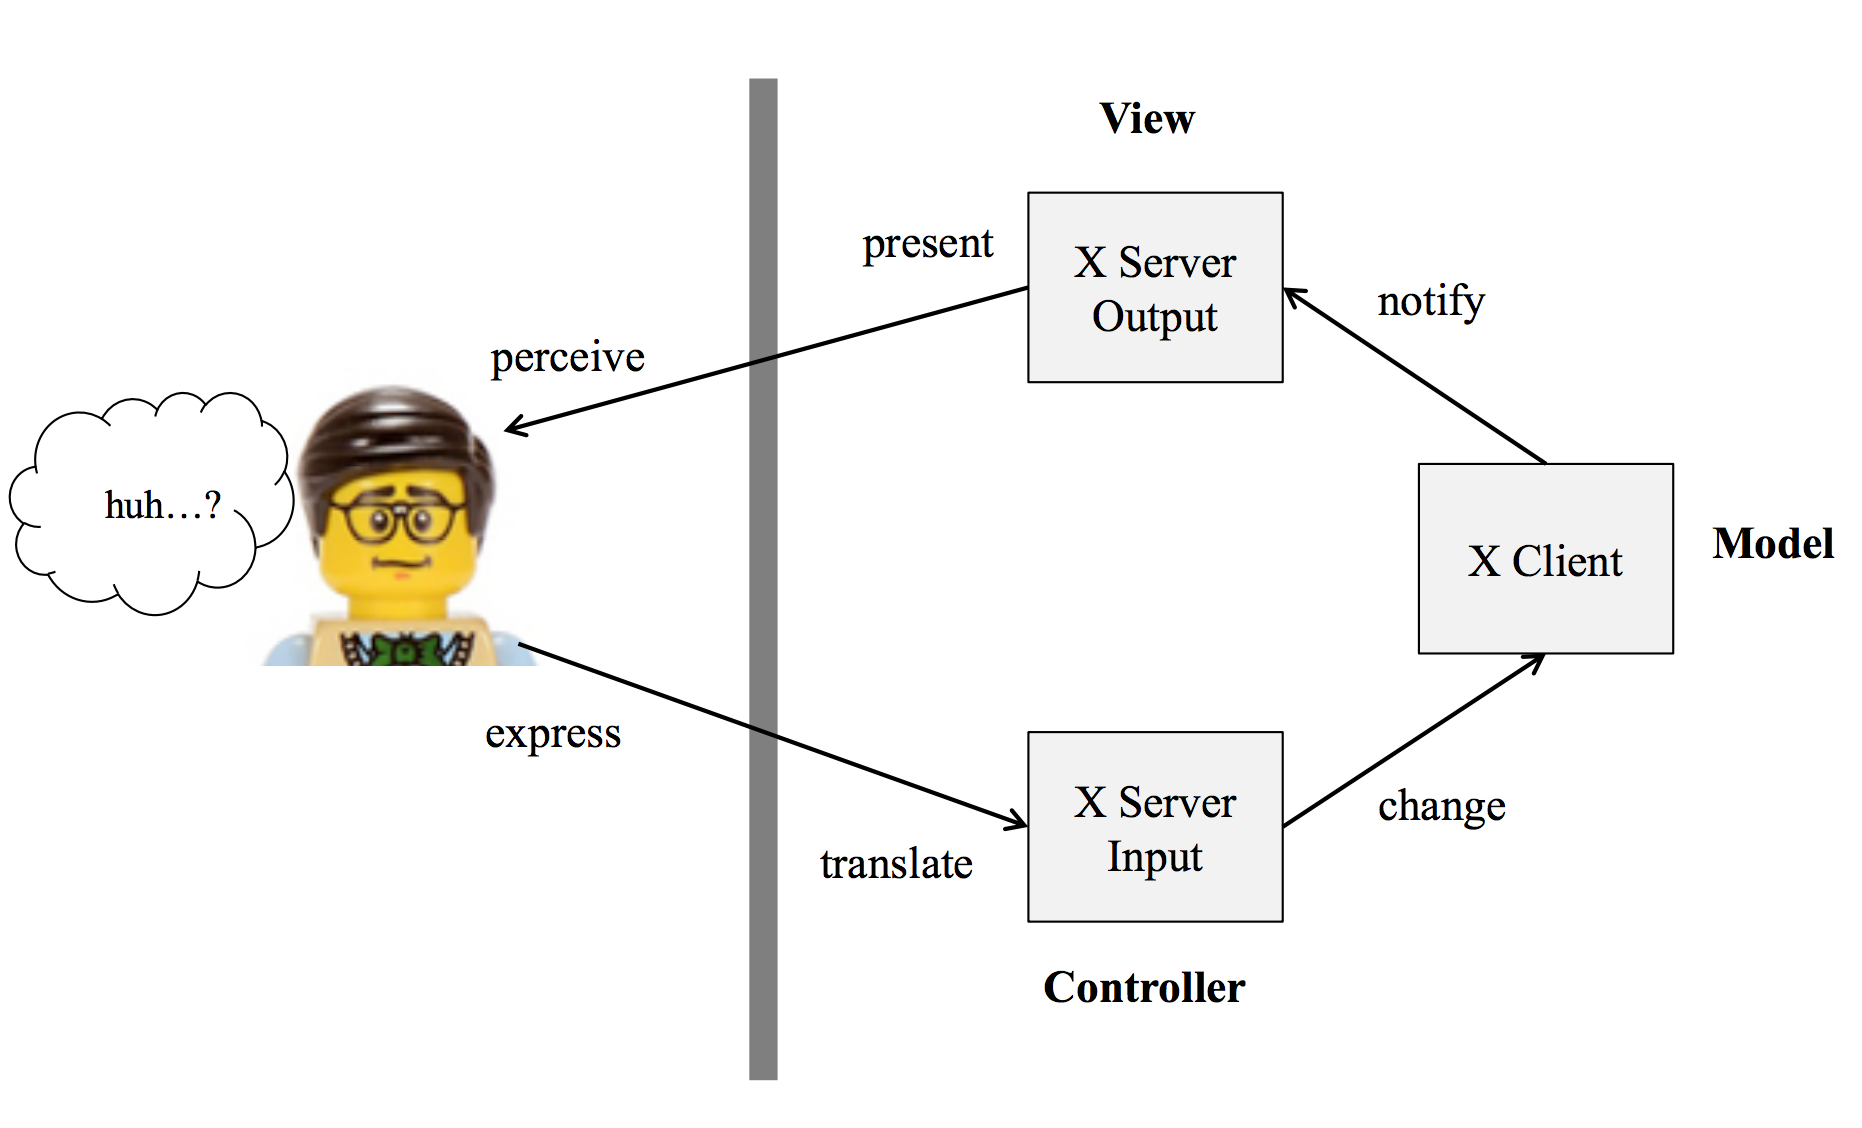
\includegraphics[width=0.6\textwidth]{res/mvc_x11.png}

# X11 is a \textbf{base windowing system}: \\
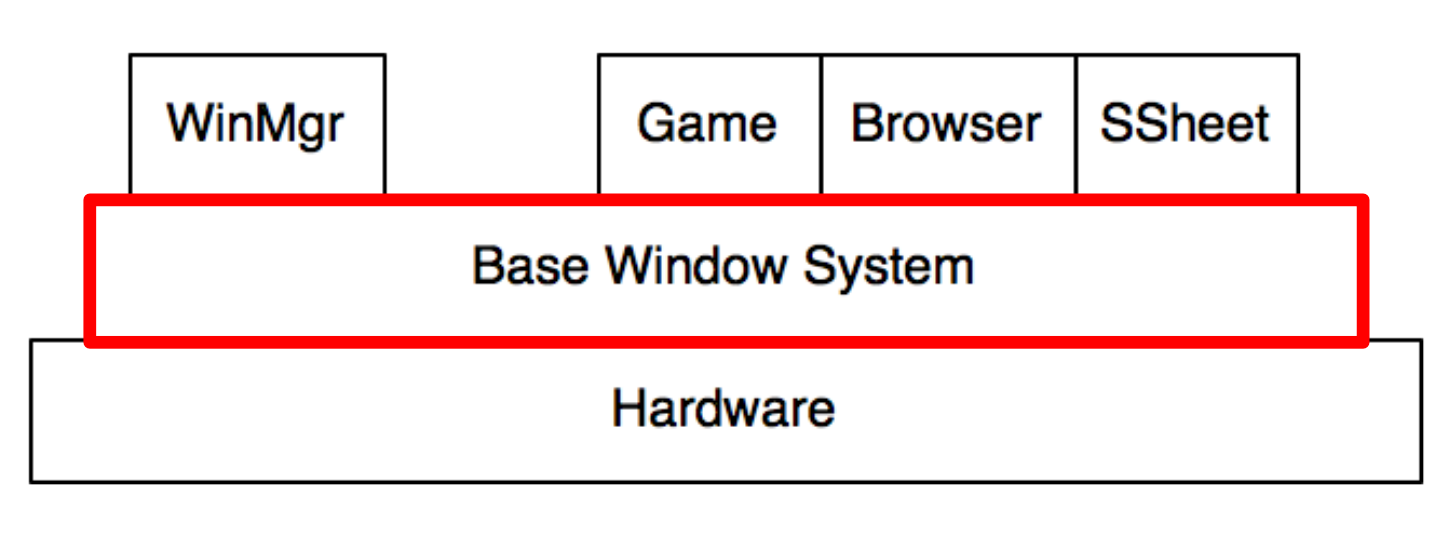
\includegraphics[width=0.4\textwidth]{res/bws.png}
## A standard/protocol for creating windows, low-level graphical output, and user input
## Does \un{not} specify the style of each application's UI
## Provides each application with a window and manages its access
## Each application (only) owns a \un{canvas}; shielded from details such as visibility, other windows

## Some \un{design goals of X11/BWS}:
### Display- \& device- independent
### Supports multiple overlapping \& resizable windows
### A display may have multiple screens (monitors) and a window may span multiple screens
### High-performance, high-quality text, 2D graphic \& imaging

# \textbf{Window manager}:
## Provides interactive components (e.g. menus, close button, resizing)
## Separation of the WM from the BWS enables many alternative ``look and feels'' \\
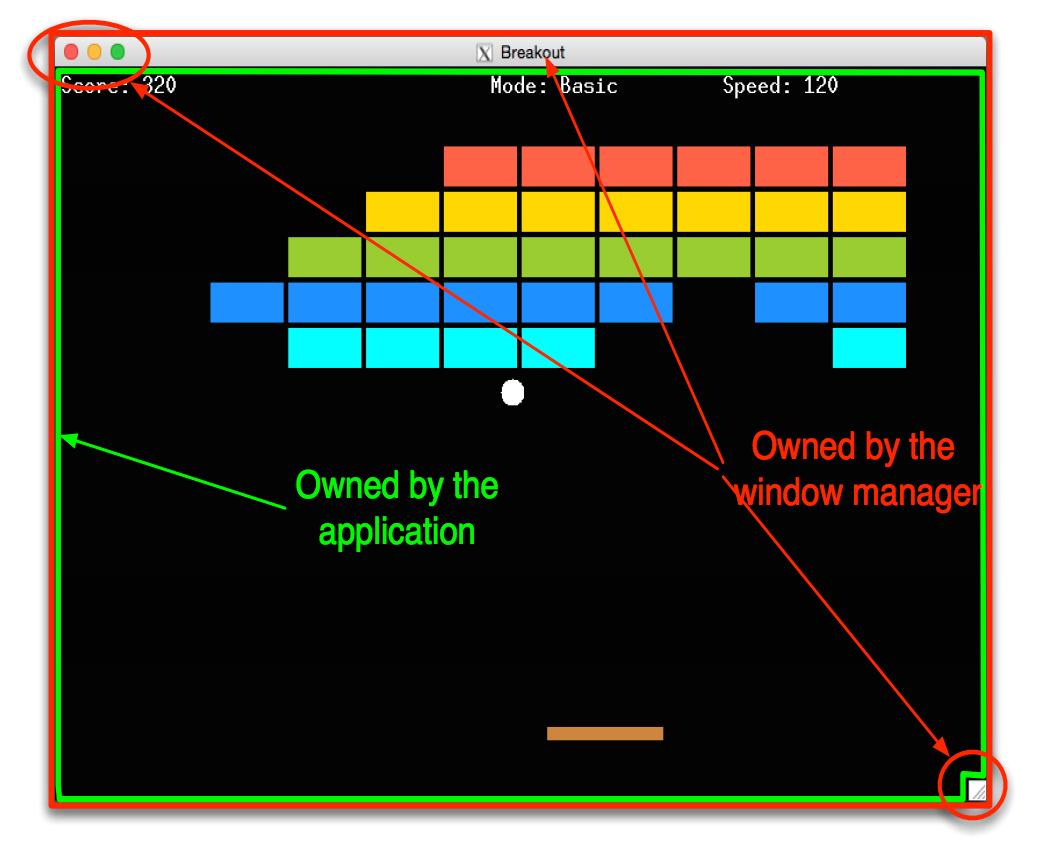
\includegraphics[width=0.45\textwidth]{res/wm.png}

# \textbf{Drawing}
## Three conceptual drawing models:
### Pixel (e.g. images)
### Stroke (e.g. lines, outlines of shapes)
### Region (e.g. text, filled shapes)

## X11 uses \un{graphics contexts} to store drawing options/parameters -- stored on X server

## \textbf{Clipping}: exposing only a particular region (specified by a \un{mask}) of an underlying image
### Only exposed area is repainted -- more efficient

## \textbf{Painter's Algorithm}: draw shapes in layers from back to front to create composite shapes

\end{easylist}


% ============================

\subsection*{Widgets}
\begineasylist

# \textbf{Widgets}: parts of an interface that have their own behaviour
## Control their own appearance; recieve and handle their own events
## Design goals: 
### \un{Complete} -- covers wide range of functionality
### \un{Consistent} -- look-and-feel across components
### \un{Customizable} -- developers can extend functionality

\hspace{-5em}
\begin{tabular}{|l|l|}
\hline
\begin{minipage}[t]{0.45\textwidth}
\textbf{Heavyweight widgets}:
    \begin{itemized}
    \item Wrappers around OS's native GUI \& windowing system 
    \item e.g. Java AWT
    \end{itemized}
    \vspace*{0.5em}
\end{minipage}
&
\begin{minipage}[t]{0.45\textwidth}
\textbf{Lightweight widgets}:
    \begin{itemized}
    \item OS provides top-level window in which widgets are drawn
    \item Toolkit is responsible to passing events to widgets
    \end{itemized}
    \vspace*{0.5em}
\end{minipage}  \\
\hline
\begin{minipage}[t]{0.45\textwidth}
Advantages:
    \begin{itemized}
    \item Events passed directly to OS/BWS
    \item Preserves the OS look-and-feel
    \end{itemized}
    \vspace*{0.5em}
\end{minipage}
&
\begin{minipage}[t]{0.45\textwidth}
Advantages:
    \begin{itemized}
    \item Consistent look-and-feel across platforms
    \item Consistent widget set across platforms
    \end{itemized}
    \vspace*{0.5em}
\end{minipage}  \\
\hline
\begin{minipage}[t]{0.45\textwidth}
Disadvantages:
    \begin{itemized}
    \item OS-specific programming
    \item Small set of common widgets across different platforms
    \end{itemized}
    \vspace*{0.5em}
\end{minipage}
&
\begin{minipage}[t]{0.45\textwidth}
Disadvantages:
    \begin{itemized}
        \item May appear ``non-native''
    \end{itemized}
    \vspace*{0.5em}
\end{minipage}  \\
\hline
\end{tabular} \\

# Widgets as logical input devices \\
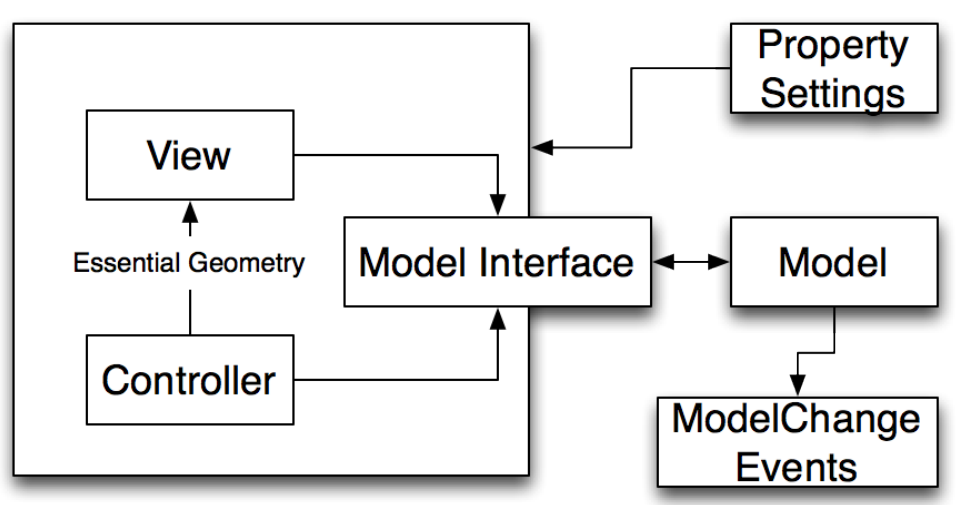
\includegraphics[width=0.4\textwidth]{res/mvc_widget.png}
## Characteristics:
### \un{Model} manipulated by the widget (e.g. number, text)
### \un{Events} generated by the widget (e.g. changed)
### \un{Properties} (behaviour and appearance) of the widget (e.g. colour, size, allowed values)
### e.g. radio button: model = \emph{Boolean}; events = \emph{changed}; properties = \emph{size, colour etc.}
\end{easylist}

% ============================

\subsection*{Events}
\begineasylist

# \textbf{Event-driven programming}: flow of program is determined by \un{events} such as user input (key press, mouse click, input focus change) or messages from other programs/threads
## Objective: need to map input from real-word devices $\rightarrow$ actions within a system
## Events are pushed into an \un{event queue} by the BWS (i.e. event capture)
## Implementation in X11:
### Use \texttt{XSelectInput()} and event masks to register/subscribe to types of events \& filter out unneeded events
### Use \texttt{XNextEvent()} to dequeue the next event; \emph{may block if no events}
#### Use \texttt{XPending()} to check for \# of events before dequeueing
### Should dequeue \emph{all events} before repainting to avoid input lag
### Should subtract time spent in event loop from \texttt{sleep()} to maintain consistent FPS
### Should draw all images to a \emph{buffer} (\texttt{XCreatePixmap()}), then copy the buffer onto the screen in one go (\texttt{XCopyArea()}) (aka. \un{double buffering})
#### Avoids displaying an intermediate image (i.e. flickering)
\\\\
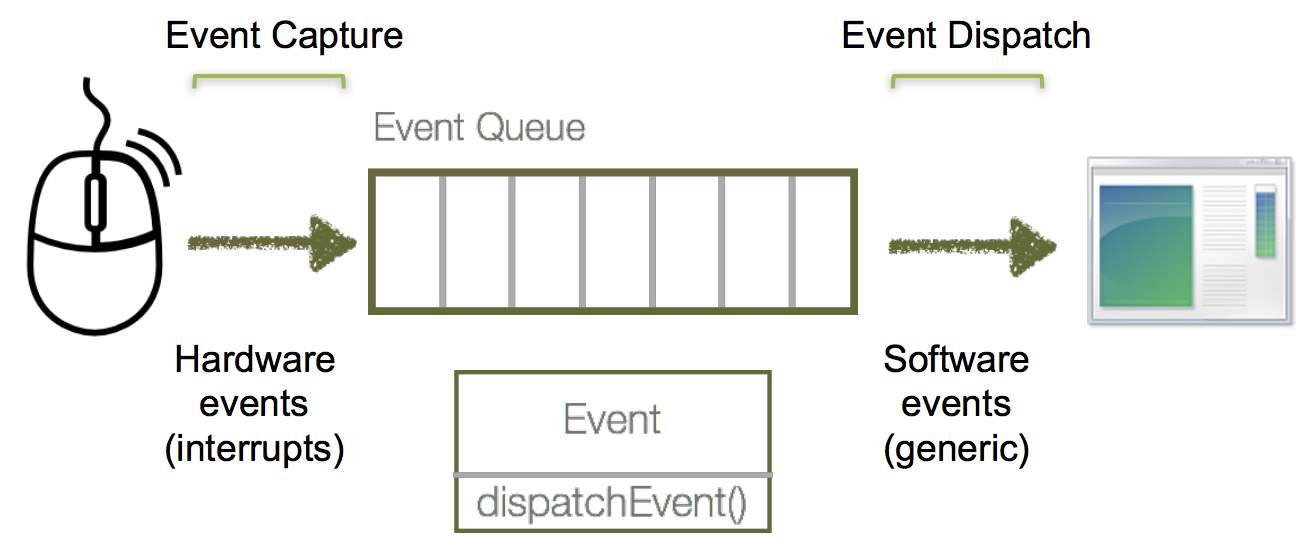
\includegraphics[width=0.5\textwidth]{res/event_queue.png}

# \textbf{Event dispatch}: dequeueing events from event queue and pushing to appropriate applications

# \textbf{Interactor tree} -- hierarchy of containers and their nested widgets

# \textbf{Positional dispatch} -- input sent to widget under mouse cursor location
## \un{Bottom-up dispatch}:
### Event is routed to leaf (lowest) widget in interactor tree; can pass to parent
#### e.g. sometimes may be better for the container of a widget to handle the event
### Advantage: event does not have to traverse through entire tree to arrive at widget
## \un{Top-down dispatch}:
### Event is routed to highest-level node that contains mouse cursor; can pass to child
### Advantages:
#### Parent widget can enforce policies (e.g. make children view-only)
#### Easy event logging (as it traverses down through the tree)
## Pure positional dispatch can be problematic
### e.g. mouse-down inside a button, mouse-up outside
### e.g. dragging scrollbar but mouse moves out of scrollbar

# \textbf{Focus dispatch}
## At most one widget each can be in keyboard \& mouse focus at a given time
## Focus dispatch also needs positional dispatch to change focus (i.e. mouse click)
## Accelerator keys (i.e. keyboard shortcuts) can bypass focus dispatch -- they're handled before widget receives events

\hspace{-2em}
\begin{tabular}{|l|l|}
\hline
\begin{minipage}[t]{0.45\textwidth}
\textbf{Heavyweight toolkits}:
    \begin{itemized}
    \item BWS has visibility to all widgets
    \item Can use top-down or bottom-up dispatch
    \end{itemized}
    \vspace*{0.5em}
\end{minipage}
&
\begin{minipage}[t]{0.45\textwidth}
\textbf{Lightweight toolkits}:
    \begin{itemized}
    \item BWS only has visibility to application window
    \item Toolkit then dispatches event to widget
    \item Can only use top-down dispatch
    \end{itemized}
    \vspace*{0.5em}
\end{minipage}  \\
\hline
\end{tabular} \\

# \textbf{Event handling}: interpreting events in widget's application code
## Design goals of event-code binding:
### Easy to understand
### Easy to implement
### Easy to debug
### Good performance

## Event loop \& switch statement (X11):
### All events are consumed in one event loop
### Switch statement selects the appropriate code for each event
### Downsides: switch statement needs to encompass every type of event (too many!)

## Inheritance binding (Java, OS X):
### Events are dispatched to base widget class with predefined event handling methods
### Child widget overrides methods with custom behaviour
### Downsides:
#### Event handling code in application logic (child widget) -- no separation of concerns
#### Difficult to add new events

## Listener binding (Java):
### \un{Interface binding} -- widget class implements event listener interfaces

\hspace{2em} \texttt{public class A implements Listener \{ // implement all methods \}}

### \un{Object binding} -- widget class holds listener objects (implement listener interface as a nested class)
#### Event handling \& application code are decoupled

\texttt{this.addListener(new Listener() \{ // implement all methods \});}

### \un{Adapter pattern} -- widget class holds adapter objects (class with boilerplate implementations)
#### Custom adapter only needs to extend methods that are used

\texttt{this.addListener(new ListenerAdapter() \{ // override some methods \});}

## Delegate binding (.NET):
### Delegates ``point'' to a method (or methods); invoking delegate calls all associated methods

\hspace{2em} \texttt{delegate = object.Method1; delegate += object.Method2; delegate(args);} \\

\end{easylist}


% ============================

\newpage
\subsection*{Layouts}
\begineasylist

# \textbf{Dynamic layout} -- dynamically adjusts screen composition
## Provides spatial layout for widgets in a container
## Handles container resize by adjusting location, size, visibility or look-and-feel of widgets
# Widgets may define constraints for size (e.g. min, preferred, max), position (e.g. anchors)
# \un{Layout managers} provide algorithms to size \& position widgets

# \textbf{Composite pattern} -- group/container of widgets and individual widgets are treated uniformly
## Widgets are organized in a tree hierarchy

# \textbf{Strategy pattern} -- abstract out the algorithm so that it can be changed at run-time
## Layout manager can employ different layout strategies

# Types of layouts:
## \un{Fixed} -- widgets have fixed size \& position
### e.g. set \texttt{LayoutManager} to null

## \un{Intrinsic size} -- parent widget's size depends \emph{solely} on contained widgets
### Bottom-up approach -- query each child widget for exact size, then set size for parent
### e.g. \texttt{BoxLayout}, \texttt{FlowLayout}

## \un{Variable intrinsic size} -- widget size depends on both parent and contained widgets' preferred sizes
### Both bottom-up \& top-down approach
### e.g. \texttt{GridBagLayout}, \texttt{BorderLayout}

## \un{Struts and Springs} -- layout specified by contraints and anchors
### Strut widgets are fixed in size; spring/glue widgets stretch to fill space
### e.g. \texttt{SpringLayout}

\end{easylist}


% ============================

\subsection*{Graphics \& Transformations}
\begineasylist

# \textbf{NOTE}: origin is located at the \un{top-left} when discussing graphics \& transformations

# \textbf{Shape model} -- data needed to draw a primitive shape (array of points, colour, location etc.)

# \textbf{Affine transformations}:
## \un{Translation}: add scalar to $x$ and/or $y$ component
## \un{Scaling}: multiply $x$ and/or $y$ components by scalars
## \un{Rotation} (about the origin): $x' = x\cos(\Theta) - y\sin(\Theta)$, $y' = x\sin(\Theta) + y\cos(\Theta)$

## Order of operations: scale $\rightarrow$ rotate $\rightarrow$ translate
### $x' = s_x(x\cos(\Theta) - y\sin(\Theta)) + t_x$
### $y' = s_y(x\sin(\Theta) + y\cos(\Theta)) + t_y$
### Since scaling \& rotation are about the origin, should \un{translate to origin first}, and translate back after scaling/rotation
## Translation can't be done using $2 \times 2$ matrix -- use \un{homogeneous coordinates}
### $[x, y, w]$ represents a point at $[x/w, y/w]$; e.g. $[1, 2, 1] = [2, 4, 2]$
## \textbf{Affine transformation matrix} (transformations are applied right to left $\leftarrow$)
\[
    \begin{bmatrix} x' \\ y' \\ 1 \end{bmatrix}
    =
    \begin{bmatrix}
        1 & 0 & t_x \\
        0 & 1 & t_y \\
        0 & 0 & 1
    \end{bmatrix}
    \begin{bmatrix}
        \cos(\Theta) & - \sin(\Theta) & 0 \\
        \sin(\Theta) & \cos(\Theta) & 0 \\
        0 & 0 & 1
    \end{bmatrix}
    \begin{bmatrix}
        s_x & 0 & 0 \\
        0 & s_y & 0 \\
        0 & 0 & 1
    \end{bmatrix}
    \begin{bmatrix} x \\ y \\ 1 \end{bmatrix}
\]

# \textbf{Scene graph} -- each component has a transformation matrix \& draws its child components relative to itself
## The interactor tree is a type of scene graph
## Each component has a transformation matrix (describes its location relative to parent)
### Each componnt paints itself, then
### Combine its matrix with child component's matrix, and tells child to paint itself using combined matrix

# Benefits of geometric manipulation:
## Allows reuse of objects (create multiple instances via transformations)
## Allows specification of object in its own coordinate system (e.g. relative to parent)
## Simplifies repositioning of object after change (e.g. moving an object in animation)

# Coordinates given by events need to be transformed as they traverse the interactor tree
## e.g. for \un{inside tests/hit detection}, mouse event coordinates must be transformed into a model's local coordinates 
## Transforming \un{mouse $\rightarrow$ model} coordinates
### Only one transformation (of the mouse event) -- take the inverse of model's affine matrix
## Transforming \un{model $\rightarrow$ mouse} coordinates
### Many transformations (of all objects in the scene) in order to find which one the mouse is inside of



% ============================

\end{easylist}

\subsection*{Model-View-Controller}
\begineasylist

# \textbf{MVC} -- multiple views \emph{loosely coupled} with the underlying data model
## Developed for Smalltalk-80 by Trygve Reenskaug
## Tight coupling of data \& presentation prevents easy modification and extension
## \un{Separation of concerns} enables:
### Alternate forms of interaction/presentation with the same data
### Multiple, simultaneous views of data
### Easy testing of data manipulations that are independent of the UI
## \un{View} \& \un{controller} can access the \un{model} through its interface; model only knows about the view
### Controller $\rightarrow$ (notifies) $\rightarrow$ Model
### View $\rightarrow$ (queries) $\rightarrow$ Model
### Model $\rightarrow$ (updates) $\rightarrow$ View
### Controller \& view are \un{tightly coupled} in practice 
#### Controller is just part of the view class that calls the model's interface based on input

# MVC is an instance of the \textbf{observer pattern}
## Allows objects to communicate without knowing each others' specific types
## In Java, the view implements \texttt{Observer} (like \texttt{IView}); model extends \texttt{Observable} \\
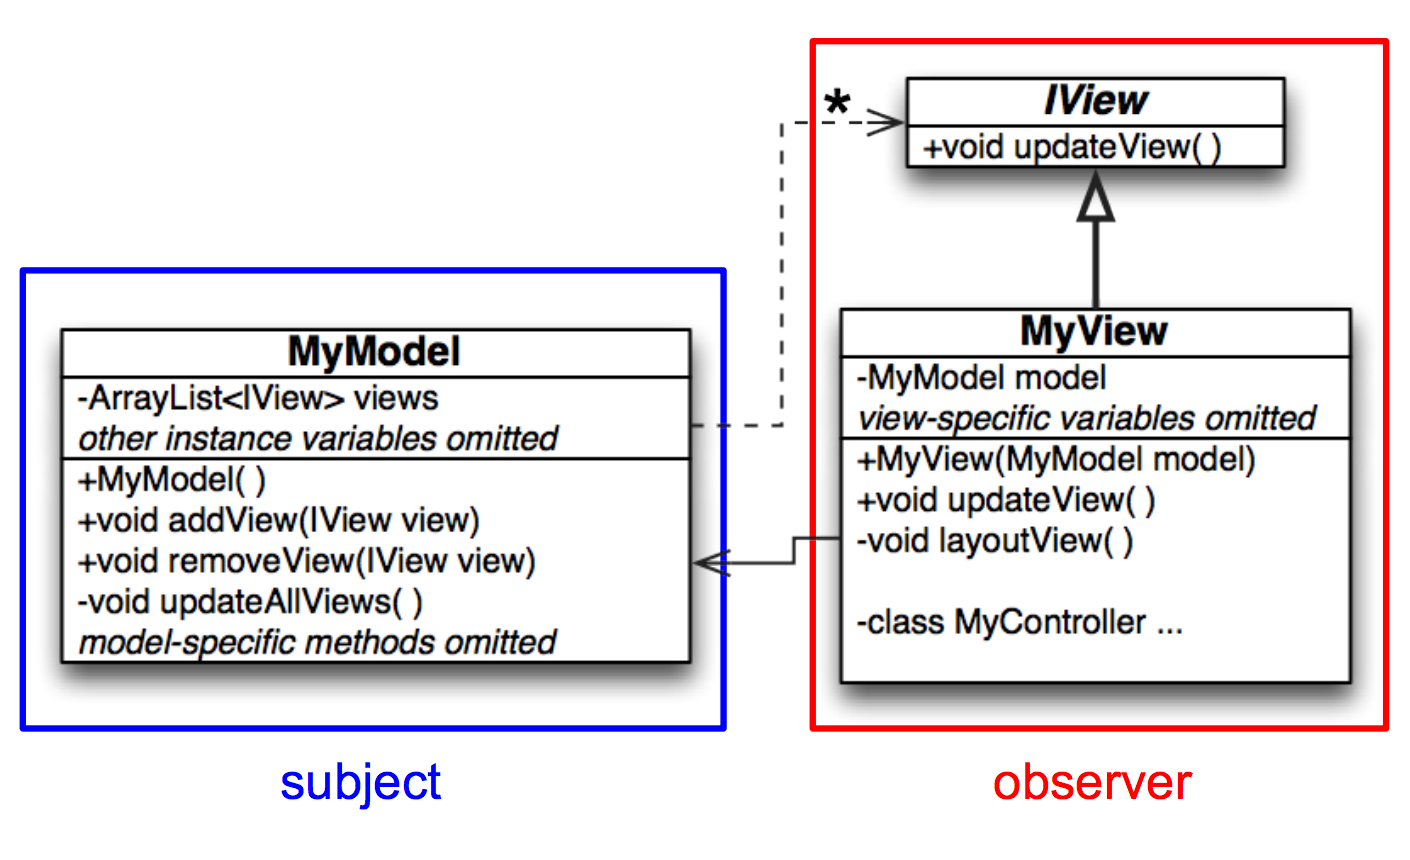
\includegraphics[width=0.6\textwidth]{res/mvc_observer.png}


\end{easylist}


% ============================

\subsection*{Input}
\begineasylist

# Computer input can be classified by sensing method (e.g. mechanical, motion, contact), continuous vs. discrete, degrees of freedom
# Specific vs. general input
## Specific inputs are optimized for certain tasks (but can't do others); general inputs can be adapted to many tasks (but lack accuracy/optimization)
# \textbf{Text input}
## QWERTY has many \emph{perceived} inefficiencies; Dvorak attempts to address these problems, but actual difference in speed is discernible
## Portability (smaller, lower-profile keys) of keyboards also interfere with typing performance
## Soft/virtual keyboards lack haptic feedback, but improves aethestics -- good for when the amount of input is limited

# \textbf{Positional input}
## \un{Isometric} (force) vs. \un{isotonic} (displacement) sensing
### Device senses displacement (mouse) or force (joystick)
## \un{Position} vs. \un{rate} control
### Change in input device maps to change in position (mouse) or speed (joystick)
### Usually, isometric $\rightarrow$ rate, isotonic $\rightarrow$ position
## \un{Absolute} vs. \un{relative} position
### 1:1 mapping between input \& output position (touchscreen) or non-1:1 mapping (mouse)
## \un{Direct} vs. \un{indirect} contact
### Input takes place on the same surface as output (touchscreen) or on a different surface (mouse)
## Dimensions sensed -- 1 (dial) vs. 2 (mouse) vs. 3 (Wiimote)

## Control-display gain = ratio between the movement speeds of pointer on screen \& physical mouse

# \textbf{Keystroke Level Model} (KLM):
## Use operators to estimate how long an input task should take
### Keystroke (K), pointing (P), mouse button press (B), hand move between mouse \& keyboard (H), mental preparation (M)
### M is only needed when user needs to think, e.g. initiate a task, make a decision, or if they are a novice

## Advantages:
### Easy to model; can be done before an interface is actually built
## Disadvantages:
### Estimates can be out of date or inherently variable
### Doesn't model errors and learning time

# \textbf{Fitts' Law}:
## Predictive model for 2D pointing time, especially robust for modelling human hand movements
## In general, longer distance \& smaller target $\rightarrow$ longer time
\[ MT = a + b\log\left(\frac{D}{W} + 1\right) \]
### $MT$ = movement time
### $D$ = distance from starting point $\leftrightarrow$ centre of target
### $W$ = constraining size (e.g. width) of target
### $a, b$ = some parameters of the input device
### $b$ = index of performance ($IP$) $\approx MT/ID$
### $\log(D/W + 1)$ = index of difficulty ($ID$)

## \un{Visual space}: how something appears to move on-screen
## \un{Motor space}: how movement feels relative to input
## Cursor speeds can be manipulated to make objects seem bigger in motor space (stickier)

# \textbf{Steering Law}:
## When steering through a path between boundaries (e.g. context menus):
\[ T = b \frac{D}{W} \]
## Time to travel a complex path = sum of the times taken to travel each small path
## When steering between boundaries, distance \& width have greater influence on difficulty

\end{easylist}


% ============================

\subsection*{Direct Manipulation}
\begineasylist

# \textbf{Domain objects} -- object of interest; data/attribute (model)

# \textbf{Interaction instrument} -- used by user to manipulate domain objects
## In turn manipulated through physical actions by user

# Spatial activation -- instrument put under user control due to cursor movement
## Cost = cursor movement distance

# Temporal activation -- instrument put under user control due to some former action; enters a state
## Cost = sequence of previous actions/steps required

# Degree of indirection:
## Spatial offset (e.g. object follows mouse drag) \& temporal offsets (e.g. immediate response)

# Degree of integration:
## Degrees of freedom of the instrument vs. input device
## e.g. 2D mouse + 1D scrollbar (higher degree) vs. 2D mouse + 3D model (lower degree)

# Degree of compatibility:
## Similarity between physical action on instrument vs. response in object
## e.g. dragging (high similarity) vs. dialog box (low similarity)

# \textbf{Direction manipulation} attempts to make user actions resemble real-world actions on objects
## Visible \& continuous representation of the domain objects and actions
## Objects are manipulated by physical actions, e.g. clicking/dragging
## Effects of operations on objects are immediately visible
## Actions should be reversible
## Allows users to feel like they are interacting directly with domain objects rather than an interface

\bigskip
# DM feature: \textbf{Undo/Redo}

## Enables exploratory learning; lets the user recover from errors
## \un{Design decisions}:
### Undoable actions
### UI state after undo
### Granularity
### Scope

## \un{Forward undo} -- apply CRs (change records) forwards from some baseline document
## \un{Reverse undo} -- save reverse CRs and apply them in reverse

## \un{Memento pattern} -- save snapshots of (entire or incremental) document state
## \un{Command pattern} -- save commands (or reverse commands)

## e.g. Java uses reverse undo + command
### User issues command $\rightarrow$ push onto undo stack, clear redo stack
### Undo $\rightarrow$ pop from undo, perform reverse command, push onto redo
### Redo $\rightarrow$ pop from redo, perform command, push onto undo

\bigskip
# DM feature: \textbf{Clipboard}

## Cut + paste/drag + drop allows for easy data transfer within and between applications
## Copy $\rightarrow$ paste format may be different (e.g. many image formats)
### Application indicates what formats the data on clipboard is available in

## For large amounts of data, may put a reference on clipboard instead (instead of making a copy)
### Saves memory
### But must create a copy if data is changed, or application is closed

## Owned/maintained by the \un{window system}, not individual applications

\end{easylist}


% ============================

\newpage
\subsection*{Responsiveness}
\begineasylist

# Responsiveness $\neq$ performance
## Performance = computations per unit time
## Responsiveness = compliance with human time requirements (\un{deadlines})

\end{easylist}


% ============================

\subsection*{Touch Interfaces}
\begineasylist

\end{easylist}

\end{document}
